% Bài báo nghiên cứu, bản tiếng Việt, mẫu IEEE hội nghị (IEEEtran).
% Biên dịch: cd reports/research_paper && latexmk -pdf paper_vi.tex   (hoặc xelatex/pdflatex, chạy 2 lần)
% Hình do ../make_figures.py sinh ra (bản _vi) từ nhật ký chạy thật trong docs/data/.
\documentclass[conference]{IEEEtran}
\IEEEoverridecommandlockouts

\usepackage{iftex}
\ifPDFTeX
  \usepackage[utf8]{inputenc}
  \usepackage[T5]{fontenc}
  \usepackage{lmodern}
\else
  \usepackage{fontspec}
\fi
\usepackage{cite}
\usepackage{amsmath,amssymb}
\usepackage{graphicx}
\usepackage{booktabs}
\usepackage{array}
\usepackage{url}
\usepackage{textcomp}

\renewcommand{\figurename}{Hình}
\renewcommand{\tablename}{Bảng}
\renewcommand{\abstractname}{Tóm tắt}
\renewcommand{\IEEEkeywordsname}{Từ khóa}
\renewcommand{\refname}{Tài liệu tham khảo}
\graphicspath{{../figures/}}
\renewcommand{\arraystretch}{1.12}

\begin{document}

\title{A Vision-Based Dual-Mode Hand Gesture Interface for Simultaneous GUI Interaction and Teleoperation of a Four-Wheel Omnidirectional Mobile Robot}

\author{\IEEEauthorblockN{Tai Nguyen Anh}
\IEEEauthorblockA{{[Khoa, trường]}\\
{[Thành phố, quốc gia]}\\
{[địa chỉ email]}}}

\maketitle

\begin{abstract}
Điều khiển từ xa robot di động bằng cử chỉ tay thường chỉ dừng ở các lệnh chuyển động, nên người vận hành vẫn phải quay lại chuột hoặc bàn phím để đổi chế độ, chỉnh tốc độ hay bấm dừng khẩn cấp. Bài báo trình bày một hệ thống chi phí thấp trong đó một camera laptop phục vụ cả hai việc: tay thuận điều khiển con trỏ ảo trên giao diện web, còn tay không thuận ra lệnh cho ba bậc tự do phẳng $(v_x, v_y, \omega)$ của robot đa hướng bốn bánh cấu hình chữ X. Trên laptop, một đường xử lý hình học đặt trên các điểm mốc bàn tay của MediaPipe gán vai trò hai tay và sửa trực tuyến nhãn trái/phải bị đảo do ảnh lật gương, rồi làm mượt con trỏ bằng bộ lọc One-Euro. Trên bộ điều khiển ESP32 của robot, bốn vòng độc lập 100\,Hz kết hợp feedforward bù vùng chết riêng cho từng bánh với bộ điều khiển PI có khâu tích phân bị đóng băng khi tăng tốc và bão hòa. Hệ thống được đánh giá trên $13{.}080$ chu kỳ điều khiển đã ghi ($2{.}026$\,s) từ ba lần chạy trên sàn. Vòng thị giác chạy $29{,}9$ khung/giây với thời gian suy luận điểm mốc trung bình $18{,}5$\,ms; độ trễ khứ hồi UDP qua điểm truy cập Wi-Fi do chính robot phát có trung vị $6{,}6$--$8{,}1$\,ms (phân vị 95 là $16$--$26$\,ms); sai số tốc độ bánh trung bình khi có tải là $1{,}5$--$3{,}2$\,\% tốc độ tối đa; và chuyển động thân robot tái tạo từ encoder lệch so với lệnh $0{,}1$--$2{,}5$\,\%. Hai cơ chế con trỏ có vẻ hiệu quả trên bàn tay mô phỏng, bộ lọc One-Euro và neo điểm click, lại cho ít hoặc không có lợi ích trên bàn tay thật (rung giảm $5$\,\%; độ lệch click không giảm; được trình bày như kết quả âm). Mọi kết quả đến từ một robot và một người vận hành, và chưa có khảo sát người dùng.
\end{abstract}

\begin{IEEEkeywords}
robot di động đa hướng, giao diện cử chỉ tay, tương tác người--robot, điều khiển từ xa, bộ lọc One-Euro, điều khiển feedforward, ESP32
\end{IEEEkeywords}

%--------------------------------------------------------------------
\section{Giới thiệu}
Robot di động đa hướng (OMR) dùng bánh omni hoặc mecanum chuyển động holonomic: tịnh tiến tiến, ngang hoặc chéo và xoay tại chỗ với ba vận tốc độc lập $(v_x, v_y, \omega)$ \cite{siegwart2011}. Sự tự do này khiến điều khiển từ xa khó hơn, vì người vận hành phải ra lệnh cho ba đại lượng ghép cặp trong khi vẫn giám sát robot qua giao diện đồ họa.

Giao diện không tiếp xúc dựa trên camera và bộ dò điểm mốc bàn tay như MediaPipe Hands \cite{zhang2020} hấp dẫn vì không cần thiết bị đeo. Thiết kế phổ biến ánh xạ một bàn tay sang một tập nhỏ các lệnh chuyển động rời rạc. Với thiết kế đó, các tác vụ thuộc giao diện giám sát (đổi chế độ điều khiển, chỉnh thanh trượt tốc độ, bấm dừng khẩn cấp) thường vẫn cần chuột hoặc bàn phím vật lý. Dùng đầu ngón trỏ làm con trỏ chuột cũng có vấn đề riêng: rung tần số cao khi giữ yên tay, và đầu ngón trỏ bị dịch khi duỗi thêm ngón thứ hai để click. Cả hai hóa ra nhỏ trong các phép đo bàn tay thật của chúng tôi (mục~IV-B).

Ở phía chấp hành, ESP32 chi phí thấp với cầu H lưỡng cực L298N có vùng chết lớn và các động cơ không đồng đều. Ở robot của chúng tôi, ngưỡng ma sát tĩnh giữa các bánh chênh nhau $2{,}7$ lần ($5{,}5$\,\% đến $14{,}8$\,\% PWM), nên cùng một PWM vòng hở làm bốn bánh quay với tốc độ khác nhau và robot bị xoay lệch khi ra lệnh đi thẳng.

Bài báo mô tả một hệ thống giải quyết cả hai phía bằng một camera và một vi điều khiển. Đóng góp gồm:
\begin{enumerate}
  \item Giao diện hai bàn tay, trong đó tay thuận điều khiển toàn bộ giao diện và tay không thuận lái robot từ cùng một luồng camera, gồm bộ phân vai sửa trực tuyến nhãn trái/phải bị đảo của ảnh lật gương.
  \item Kiến trúc host--edge qua điểm truy cập Wi-Fi do chính robot phát, dùng UDP, với khóa chủ duy nhất, watchdog hai đầu và giới hạn gia tốc.
  \item Bộ điều khiển feedforward cộng PI cho từng bánh trên ESP32 với chống bão hòa có điều kiện, được nhận dạng từ đặc tính bánh xe đo được.
\end{enumerate}
Chúng tôi đánh giá đường truyền và bộ điều khiển trên các lần chạy thật đã ghi, và cũng báo cáo một kết quả âm trên bàn tay thật cho hai cơ chế con trỏ.

%--------------------------------------------------------------------
\section{Kiến trúc hệ thống và động học}
\subsection{Kiến trúc host--edge}
Hình~\ref{fig:arch} mô tả hệ thống. Laptop (host) thu hình MJPG $640\times480$ ở 30 khung/giây trong một luồng riêng chỉ giữ khung mới nhất, và chạy MediaPipe HandLandmarker hai tay trên CPU. Bộ phân vai chia các bàn tay dò được thành tay giao diện và tay lái. Tay giao diện cập nhật con trỏ, gửi qua WebSocket tới trình duyệt; tay lái được phân loại thành cử chỉ chuyển động. Vòng điều khiển 20\,Hz chọn lệnh theo chế độ đang dùng (thủ công hoặc cử chỉ), giới hạn gia tốc rồi gửi qua UDP cho robot.

Robot (edge) là ESP32 tạo điểm truy cập Wi-Fi (\texttt{omni-robot}, $192{,}168{,}4{,}1$, cổng UDP $4210$) và tắt chế độ ngủ modem. Mỗi $10$\,ms nó đọc lệnh mới nhất, áp dụng động học nghịch, chạy bốn bộ điều khiển bánh và điều khiển hai mô-đun L298N. Mỗi lệnh được xác nhận bằng một bản tin chứa, cho từng bánh, tốc độ đặt, tốc độ đo và PWM. Laptop ghi các giá trị này ở 20\,Hz vào tệp CSV.

Hai cơ chế an toàn giới hạn ảnh hưởng khi mất liên kết. ESP32 trả lệnh không nếu không có gói nào trong $300$\,ms, và chỉ nhận gói từ một địa chỉ chủ cho đến khi địa chỉ đó im lặng bằng khoảng thời gian ấy. Trên laptop, lệnh cũ hơn $0{,}4$\,s bị thay bằng không.

\begin{figure*}[!tb]
  \centering
  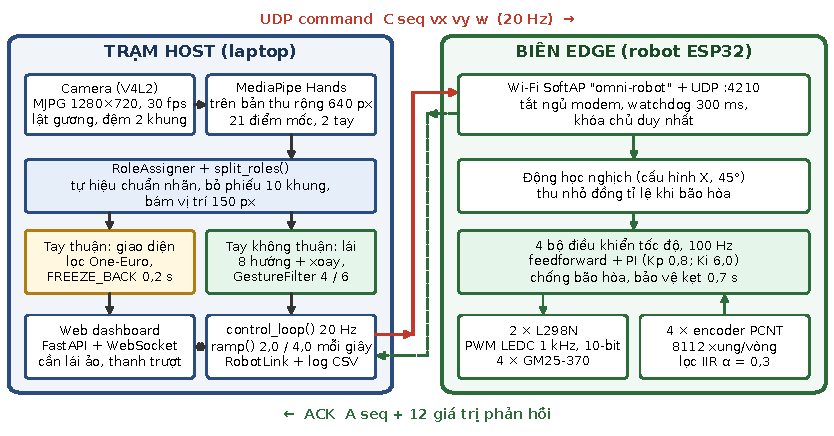
\includegraphics[width=0.86\textwidth]{fig_arch_vi.pdf}
  \caption{Kiến trúc host--edge. Đỏ liền: lệnh UDP; xanh đứt: phản hồi kèm số liệu 4 bánh.}
  \label{fig:arch}
\end{figure*}

\subsection{Mô hình động học}
Vận tốc thân theo quy ước ROS (Hình~\ref{fig:kin}): $+x$ tiến, $+y$ sang trái, $+\omega$ ngược chiều kim đồng hồ. Gọi $\mathbf{u}=[v_x, v_y, \omega]^{\top}\in[-1,1]^3$ là lệnh thân chuẩn hóa và $\mathbf{r}=[r_{tt}, r_{tp}, r_{st}, r_{sp}]^{\top}$ là tốc độ bốn bánh (trước trái, trước phải, sau trái, sau phải), trong đó $1{,}0$ ứng với $4300$ xung encoder mỗi giây. Với cấu hình chữ X $45^{\circ}$, firmware dùng
\begin{equation}
\mathbf{r}'=\begin{bmatrix}1&-1&-1\\1&1&1\\1&1&-1\\1&-1&1\end{bmatrix}\mathbf{u},\qquad
r_i=\frac{r'_i}{\max\!\left(1,\max_j |r'_j|\right)}.
\label{eq:ik}
\end{equation}
Việc chia chung giữ nguyên hướng chuyển động khi có bánh vượt giới hạn, còn cắt riêng từng bánh sẽ làm méo hướng. Các cột của ma trận trong (\ref{eq:ik}) trực giao và có bình phương độ dài bằng $4$, nên nghịch đảo giả là ma trận chuyển vị chia bốn \cite{lynch2017}, và vận tốc thân được tái tạo từ tốc độ bánh đo được $\mathbf{m}$ bằng
\begin{equation}
\begin{bmatrix}v_x\\v_y\\\omega\end{bmatrix}_{\text{đo}}=\frac14\begin{bmatrix}1&1&1&1\\-1&1&1&-1\\-1&1&-1&1\end{bmatrix}\mathbf{m}.
\label{eq:fk}
\end{equation}
Robot dùng bốn động cơ GM25-370 hộp số $1{:}78$ và encoder Hall. Đếm cả hai cạnh của cả hai kênh cho $8112$ xung mỗi vòng bánh. Ngoại vi đếm xung (PCNT) của ESP32 giải mã bằng phần cứng với bộ lọc nhiễu $12{,}5\,\mu$s \cite{esp32trm}.

\begin{figure}[!t]
  \centering
  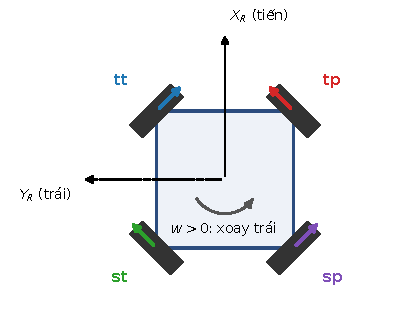
\includegraphics[width=0.62\columnwidth]{fig_kin_vi.pdf}
  \caption{Hình học cấu hình chữ X. Mũi tên là hướng đẩy của mỗi bánh khi tốc độ bánh dương.}
  \label{fig:kin}
\end{figure}

%--------------------------------------------------------------------
\section{Giao diện cử chỉ và điều khiển bánh}
\subsection{Trạng thái ngón và hướng chỉ}
Với mỗi bàn tay dùng 21 điểm mốc $p_k$. Một ngón $f$ được coi là duỗi khi đầu ngón xa cổ tay hơn khớp gần của nó theo một tỉ số không phụ thuộc khoảng cách bàn tay tới camera hay góc xoay trong mặt phẳng ảnh:
\begin{equation}
S(f)=\begin{cases}1,&\dfrac{\|p_{\mathrm{tip}(f)}-p_0\|_2}{\|p_{\mathrm{pip}(f)}-p_0\|_2}>1{,}15,\\[6pt] 0,&\text{ngược lại.}\end{cases}
\label{eq:ext}
\end{equation}
Nếu chỉ ngón trỏ duỗi, góc chỉ được đo từ gốc ngón trỏ $p_5$ đến đầu ngón $p_8$ trong mặt phẳng ảnh và chia thành tám múi $45^{\circ}$, cho tiến, lùi, trái, phải và bốn hướng chéo. Ngón trỏ và ngón giữa cùng chỉ sang trái hoặc phải là lệnh xoay. Nắm tay hoặc xòe tay thì dừng robot. \texttt{GestureFilter} cần $4$ khung liên tiếp để bắt đầu một lệnh chuyển động và $6$ khung để dừng.

\subsection{Vai trò hai tay}
Vì ảnh hiển thị đã lật gương, nhãn trái/phải của MediaPipe bị đảo so với góc nhìn người dùng. Bộ phân vai xử lý ba trường hợp. Với hai tay, vai theo thứ tự hoành độ cổ tay, và sự không khớp giữa thứ tự này với nhãn (đã đảo) cập nhật điểm $c_k=0{,}95\,c_{k-1}\pm0{,}05$; khi $c_k<-0{,}6$ thì quy ước đảo được đổi. Với một tay, nhãn được bỏ phiếu trong $10$ khung gần nhất. Nếu vừa mất một tay và cổ tay còn lại dịch dưới $150$\,px thì giữ vai cũ. Ở chế độ thủ công, nhánh lái bị tắt và bất kỳ bàn tay nào cũng là tay giao diện, nên có thể dùng toàn bộ dashboard chỉ bằng một tay.

\subsection{Con trỏ, neo điểm click và nắm thanh trượt}
Vị trí đầu ngón trỏ được làm mượt bằng bộ lọc One-Euro \cite{casiez2012} với $f_{\min}=1$\,Hz và $\beta=8$ trên toạ độ ảnh chuẩn hóa: tần số cắt $f_c=f_{\min}+\beta|\dot{x}|$ thấp khi tay yên và tăng theo tốc độ. Tay giao diện có ba tư thế: \emph{point} (chỉ ngón trỏ; con trỏ di chuyển và giữ yên $0{,}8$\,s thì click), \emph{click} (trỏ cộng giữa; bấm hoặc kéo) và \emph{idle}. Một tư thế phải kéo dài $3$ khung.

Duỗi ngón giữa có thể kéo đầu ngón trỏ lệch khỏi mục tiêu định bấm (mục~IV-B đo mức lệch này). Khi tư thế đổi từ point sang click tại thời điểm $t$, lịch sử các điểm đã lọc $H$ cho điểm neo
\begin{align}
(x_a,y_a)&=\bigl(x_j,y_j\bigr)\ \text{với}\ j=\arg\max\{t_j:\ t-t_j\ge 0{,}2\,\mathrm{s}\},\nonumber\\
(\Delta x,\Delta y)&=(x_a-x(t),\;y_a-y(t)),\label{eq:anchor}
\end{align}
và điểm tác động dùng để chọn phần tử DOM là $(a_x,a_y)=\mathrm{clamp}\bigl(x+\Delta x,\;y+\Delta y\bigr)$ trong suốt lúc click. Con trỏ hiển thị vẫn bám đầu ngón tay nên kéo vẫn di chuyển bình thường; sau khi nhả, độ lệch giảm theo hàm mũ với hằng số thời gian $0{,}15$\,s. Thanh trượt được nắm bằng cách giữ yên trên nó, sau đó di chuyển tương đối theo chuyển động ngón tay, và nhả bằng cách giữ yên lần nữa.

\subsection{Điều khiển tốc độ từng bánh}
Hai bộ giới hạn bảo vệ khỏi trượt và sụt nguồn. Trên host, lệnh thân tăng với gia tốc tối đa $2{,}0\,\mathrm{s^{-1}}$ và giảm với $4{,}0\,\mathrm{s^{-1}}$, và đi qua không trước khi đổi dấu. Trên ESP32, mục tiêu của mỗi bánh tiến tới giá trị đặt với độ dốc tối đa $4{,}0\,\mathrm{s^{-1}}$.

Ở mỗi bước $10$\,ms thứ $k$, bánh $i$ có tốc độ đo đã lọc $\omega_i(k)=0{,}7\,\omega_i(k-1)+0{,}3\,c_i(k)/4300$, với $c_i$ là số xung trên giây. Luật điều khiển, gồm số hạng feedforward cộng khâu PI có chống bão hòa có điều kiện \cite{astrom2006}, là
\begin{align}
u^{\mathrm{ff}}_i&=\operatorname{sgn}(r_i)\bigl(a_i+b_i|r_i|\bigr),\quad e_i=r_i-\omega_i,\nonumber\\
I_i&\leftarrow I_i+K_i e_i\,\Delta t\ \ \text{chỉ khi không đang tăng tốc}\nonumber\\
&\qquad\qquad\text{và chưa bão hòa},\nonumber\\
u_i&=\mathrm{clamp}\bigl(u^{\mathrm{ff}}_i+K_p e_i+I_i,\,-1,\,1\bigr),\label{eq:ctrl}
\end{align}
với $K_p=0{,}8$, $K_i=6{,}0$. Các hằng số $a_i$ và $b_i$ là đường khớp bình phương tối thiểu của PWM xác lập theo tốc độ, đo khi kê bánh lơ lửng (Bảng~\ref{tab:ff}). Bánh có PWM từ $0{,}95$ trở lên trong khi tốc độ dưới $0{,}05$ suốt $0{,}7$\,s thì bị ngắt để chống kẹt.

\begin{table}[!t]
\caption{Tham số feedforward nhận dạng được (bánh lơ lửng) và sai số bám trung bình trên sàn.}
\label{tab:ff}
\centering
\small
\begin{tabular}{lcccc}
\toprule
Bánh & $a_i$ & $b_i$ & \multicolumn{2}{c}{Sai số TB (\%)} \\
 & (PWM) & & cử chỉ v1 & hai tay v2 \\
\midrule
tt & 0,076 & 0,470 & 1,9 & 2,5 \\
tp & 0,148 & 0,594 & 2,5 & 2,6 \\
st & 0,055 & 0,453 & 1,6 & 2,3 \\
sp & 0,060 & 0,464 & 1,7 & 2,5 \\
\bottomrule
\end{tabular}
\end{table}

%--------------------------------------------------------------------
\section{Thực nghiệm}
\subsection{Thiết lập}
Host là laptop Intel Core i5-13420H (12 luồng, 15\,GB RAM) chạy Linux, Python 3.12, MediaPipe 1.2.0 (CPU) và OpenCV 5.0. Robot là ESP32 DevKit V1 với hai mô-đun L298N, bốn động cơ GM25-370 và nguồn $12$\,V. Ba lần chạy trên sàn được ghi ở $20$\,Hz (Bảng~\ref{tab:data}); hai lần đầu dùng phiên bản một tay (v1) và lần thứ ba dùng phiên bản hai tay (v2). Trong lần chạy thủ công có $389$ dòng ở chế độ cử chỉ. Các dòng ghi khi nguồn motor tắt ($53$ dòng ở lần chạy thủ công) bị loại. Chỉ dùng một người vận hành và một robot. Dashboard được mô tả trong tài liệu kỹ thuật đi kèm.

\begin{table}[!t]
\caption{Các lần chạy. RTT là độ trễ khứ hồi UDP: trung vị / phân vị 95 / lớn nhất.}
\label{tab:data}
\centering
\small
\begin{tabular}{lrrr}
\toprule
Lần chạy & Dòng & Thời gian (s) & RTT (ms) \\
\midrule
Thủ công (v1)  & 3240 & 1512 & 7,8 / 22,5 / 97 \\
Cử chỉ (v1)    & 4820 &  247 & 8,1 / 26,1 / 101 \\
Hai tay (v2)   & 5020 &  266 & 6,6 / 16,1 / 909 \\
\midrule
Tổng & 13080 & 2026\textsuperscript{a} & -- \\
\bottomrule
\multicolumn{4}{l}{\footnotesize\textsuperscript{a}Tổng các thời lượng chưa làm tròn.}
\end{tabular}
\end{table}

\subsection{Đường xử lý thị giác}
Tốc độ camera và suy luận được đo trên $359$ khung liên tiếp với vòng thu hình và dò đầy đủ, khi chưa có tay trong khung: $29{,}9$ khung/giây, thời gian suy luận điểm mốc $18{,}5$\,ms (trung bình), $18{,}2$\,ms (trung vị), $27{,}1$\,ms (phân vị 95). Chi phí khi có tay trong khung chưa được đo riêng. Đặt bộ đệm driver một khung thay vì hai làm luồng hình giảm một nửa, từ $28{,}9$ xuống $14{,}5$ khung/giây trong một phép đo trước đó với MJPG, vì camera bỏ khung khi ứng dụng đang giữ bộ đệm duy nhất.

Phần logic hình học được kiểm bằng $46$ kiểm tra tự động trên bàn tay tổng hợp (cử chỉ, tư thế, phân vai gồm cả nhãn bị đảo, con trỏ) và $49$ kiểm tra xử lý con trỏ của dashboard trong trình duyệt (Chrome không giao diện, cửa sổ $1280\times900$) (click giữ yên, click hai ngón, nắm tương đối thanh trượt, kéo cần lái, nút giữ, nhả khi mất tay); tất cả đạt ngày 12/11/2026.

Trong hai lần chạy cử chỉ thật, cử chỉ sau lọc đổi $120$ và $76$ lần; $7$ ($5{,}8$\,\%) và $5$ ($6{,}6$\,\%) lần kéo dài dưới $0{,}3$\,s, tức $94{,}2$\,\% và $93{,}4$\,\% đoạn cử chỉ ổn định theo tiêu chí này. Chưa gán nhãn xem các đoạn ngắn có phải ngoài ý muốn hay không.

\emph{Con trỏ: một kết quả âm.} Bàn tay mô phỏng cho thấy lợi ích lớn: với nhiễu Gauss $2$\,px ($200$ lần chạy có hạt giống) bộ lọc giảm $65{,}5$\,\% độ lệch chuẩn ngang của con trỏ, và neo điểm click giảm $83{,}6$\,\% độ dịch điểm tác động với ngón trỏ giật $29{,}2$\,px.

Trên bàn tay thật (script \texttt{tests/real\_hand\_eval.py}, một người, khung $640\times480$) cả hai hiệu ứng đều không tái hiện. Khi giữ yên ngón trỏ $8$\,s ($209$ khung), độ lệch chuẩn của đầu ngón thô là $2{,}26$\,px và của con trỏ đã lọc là $2{,}14$\,px ($-5$\,\%); rung thật nhiều khả năng chậm và có tương quan, mà bộ lọc thông thấp chỉnh cho nhạy không loại bỏ được (chưa kiểm tra). Với độ dịch khi click, người thử giữ yên đầu ngón (trong $3$\,px suốt $1$\,s, lần nào còn trôi bị loại) và duỗi ngón giữa $12$ lần. Đầu ngón trỏ chỉ dịch trung vị $1{,}65$\,px ($1{,}1$--$5{,}7$), so với $29{,}2$\,px trong mô phỏng, còn điểm tác động có neo dịch trung vị $4{,}15$\,px ($2{,}0$--$12{,}0$), nhiều hơn đầu ngón ở $11$ trong $12$ lần (Hình~\ref{fig:real}), nên độ lùi $0{,}2$\,s làm thêm khoảng $2{,}5$\,px thay vì loại bỏ một độ dịch. Một lần đo trước đó khi người thử không giữ yên ngón tay không được dùng. Với $12$ lần click của một người và chưa đo tỉ lệ bấm trúng, kết quả chỉ mang tính tham khảo; bán kính dwell ($30$\,px) và kích thước nút đều lớn hơn các độ dịch này nên tác động thực tế lên việc bấm nhiều khả năng nhỏ nhưng chưa kiểm chứng.

\begin{figure}[!t]
  \centering
  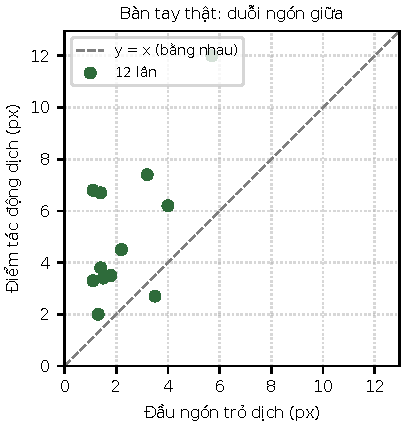
\includegraphics[width=0.78\columnwidth]{fig_real_vi.pdf}
  \caption{Bàn tay thật, 12 lần giữ yên ngón tay: độ dịch của điểm tác động so với đầu ngón trỏ thô khi duỗi ngón giữa. Điểm trên đường đứt là điểm tác động dịch nhiều hơn đầu ngón.}
  \label{fig:real}
\end{figure}

\subsection{Độ trễ đường truyền}
Độ trễ khứ hồi được đo cho từng lệnh, từ số thứ tự của lệnh UDP đến số thứ tự của bản tin xác nhận. Bảng~\ref{tab:data} và Hình~\ref{fig:rtt}(a) cho trung vị $6{,}6$--$8{,}1$\,ms và đuôi phân bố dài; giá trị tệ nhất, $909$\,ms ở lần chạy hai tay, vượt xa hạn $300$\,ms của watchdog robot nên robot sẽ dừng. Đây chỉ là độ trễ mạng khứ hồi; không gồm thu hình, suy luận và lọc cử chỉ.

Với $38$ ($26$) cử chỉ chuyển động đã chốt ở lần chạy cử chỉ v1 (hai tay v2), thời gian từ cử chỉ được ghi đến khi bánh chịu tải nhiều nhất đạt $50$\,\% mục tiêu mới có trung vị $260$\,ms ($204$--$359$\,ms) và $257$\,ms ($203$--$309$\,ms). Con số này gồm các giới hạn gia tốc có chủ ý ở mục~III-D, nên không phải độ trễ nhỏ nhất có thể, và không gồm $4$ khung ($\approx133$\,ms) cần để chốt cử chỉ.

\subsection{Bám tốc độ bánh và chuyển động thân}
Chỉ tính bám tốc độ khi lệnh không đổi $0{,}3$\,s và có độ lớn từ $0{,}1$. Bảng~\ref{tab:ff} và Hình~\ref{fig:wheel} cho sai số trung bình $1{,}5$--$3{,}2$\,\% tốc độ tối đa trên ba lần chạy. Phân vị 95 của sai số cao hơn, $4{,}4$--$4{,}8$\,\% ở lần chạy cử chỉ v1 và $6{,}1$--$7{,}4$\,\% ở lần v2, nên mốc $5$\,\% đạt theo trung bình nhưng không đạt theo đuôi ở lần v2. Bánh trước phải, có vùng chết lớn nhất, cần PWM trung bình cao nhất ($0{,}48$--$0{,}49$ so với $0{,}36$--$0{,}44$). Chúng tôi không so sánh với PID thuần hay vòng hở trên cùng quỹ đạo, nên lợi ích của bộ điều khiển đề xuất so với chúng chưa được định lượng ở đây.

Bảng~\ref{tab:odo} so lệnh với vận tốc thân tính từ encoder theo (\ref{eq:fk}) trên các đoạn có chuyển động cơ bản không đổi. Sai số theo trục chính dưới $0{,}6$\,\% khi tịnh tiến và khoảng $2{,}4$--$2{,}5$\,\% khi xoay, còn chuyển động ngoài ý muốn ở các trục khác không quá $0{,}004$. Đây là vận tốc từ encoder và không tính trượt bánh trên sàn, nên không phải sai số vị trí thật.

\begin{table*}[!t]
\caption{Lệnh so với vận tốc thân tính từ encoder (đơn vị chuẩn hóa). Sáu chuyển động đầu từ lần chạy cử chỉ v1; hai hàng chéo từ lần chạy v2.}
\label{tab:odo}
\centering
\footnotesize
\setlength{\tabcolsep}{3pt}
\begin{tabular}{lrcccc}
\toprule
Chuyển động & Mẫu & Lệnh $(v_x,v_y,\omega)$ & Từ encoder $(v_x,v_y,\omega)$ & Lệch trục chính & Trục khác lớn nhất \\
\midrule
Tiến           & 543 & (+0,472; 0; 0) & (+0,474; +0,001; +0,002) & +0,6\,\% & 0,002 \\
Lùi            & 360 & (-0,510; 0; 0) & (-0,510; -0,001; -0,001) & -0,1\,\% & 0,001 \\
Sang trái      &  96 & (0; +0,480; 0) & (+0,004; +0,482; +0,002) & +0,4\,\% & 0,004 \\
Sang phải      &  73 & (0; -0,480; 0) & (-0,003; -0,479; 0) & -0,2\,\% & 0,003 \\
Xoay trái      & 238 & (0; 0; +0,435) & (+0,003; +0,001; +0,446) & +2,5\,\% & 0,003 \\
Xoay phải      & 230 & (0; 0; -0,442) & (-0,001; 0; -0,453) & +2,4\,\% & 0,001 \\
Chéo tiến trái (v2) &  98 & (+0,308; +0,245; 0) & (+0,316; +0,256; +0,001) & -- & -- \\
Chéo tiến phải (v2) &  71 & (+0,313; -0,237; 0) & (+0,316; -0,243; -0,002) & -- & -- \\
\bottomrule
\end{tabular}
\end{table*}

\begin{figure*}[!tb]
  \centering
  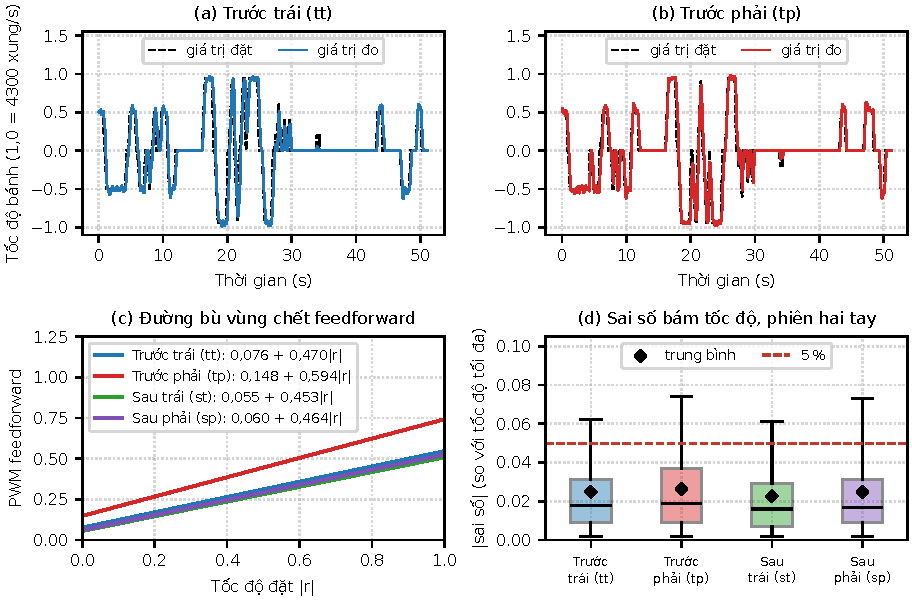
\includegraphics[width=0.86\textwidth]{fig_wheel_vi.pdf}
  \caption{Điều khiển tốc độ bánh ở lần chạy hai tay. (a), (b) Giá trị đặt và đo của hai bánh trong cửa sổ $50$\,s. (c) Đường feedforward nhận dạng được. (d) Phân bố sai số bám xác lập (râu: phân vị 5--95; hình thoi: trung bình); nét đứt đánh dấu $5$\,\%.}
  \label{fig:wheel}
\end{figure*}

\begin{figure*}[!tb]
  \centering
  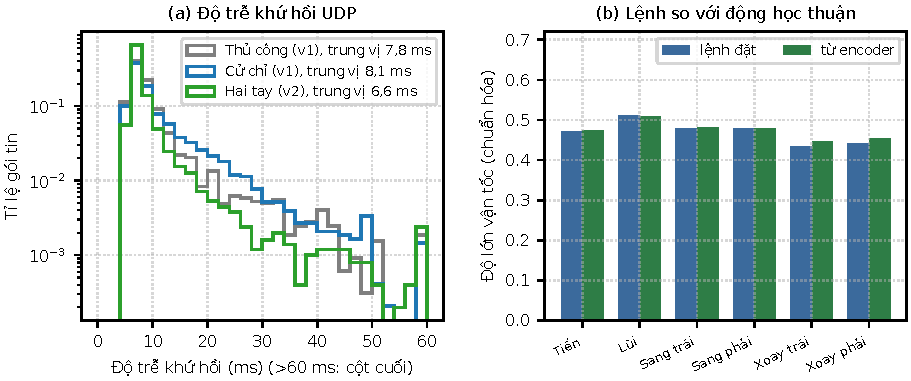
\includegraphics[width=0.86\textwidth]{fig_rtt_odo_vi.pdf}
  \caption{(a) Phân bố độ trễ khứ hồi UDP của ba lần chạy (thang log; giá trị trên $60$\,ms gom vào cột cuối). (b) Độ lớn vận tốc lệnh và vận tốc từ encoder cho sáu chuyển động cơ bản.}
  \label{fig:rtt}
\end{figure*}

%--------------------------------------------------------------------
\section{Hạn chế}
Kết quả đến từ một robot trên một sàn với một người vận hành. Chưa có khảo sát người dùng nên nhận định giao diện tiện hơn chuột chưa được kiểm chứng. Các phép đo con trỏ trên tay thật (rung, độ dịch khi click) chỉ từ một người và $12$ lần click, và chưa đo tỉ lệ bấm trúng. Thiếu phép so sánh bộ điều khiển với đường cơ sở, và tiêu chí ổn định cử chỉ không phân biệt được chuyển tiếp có chủ ý với ngoài ý muốn. Độ trễ từ lúc thu hình đến khi bánh chuyển động chưa đo đầu cuối. Hệ thống không có cảm biến vật cản: người vận hành là biện pháp an toàn duy nhất.

\section{Kết luận}
Một webcam và một ESP32 đủ để điều khiển đồng thời robot di động đa hướng bốn bánh và dashboard của nó: một tay cho giao diện và tay kia để lái. Trên các lần chạy đã ghi, độ trễ khứ hồi của đường truyền có trung vị vài mili giây, sai số tốc độ bánh trung bình là $1{,}5$--$3{,}2$\,\% tốc độ tối đa, và chuyển động thân suy ra từ encoder khớp với lệnh trong phạm vi $2{,}5$\,\%. Cơ chế neo điểm click và tham số bộ lọc cần được xem lại theo các phép đo trên tay thật. Hướng tiếp theo là khảo sát người dùng với bàn tay thật, so sánh với các bộ điều khiển cơ sở, cảm biến hướng và cảm biến vật cản.

\begin{thebibliography}{00}
\bibitem{siegwart2011} R.~Siegwart, I.~R. Nourbakhsh, and D.~Scaramuzza, \emph{Introduction to Autonomous Mobile Robots}, 2nd~ed. Cambridge, MA, USA: MIT Press, 2011.
\bibitem{zhang2020} F.~Zhang \emph{et al.}, ``MediaPipe Hands: On-device real-time hand tracking,'' arXiv:2006.10214, 2020 (CVPR Workshop on Computer Vision for AR/VR).
\bibitem{casiez2012} G.~Casiez, N.~Roussel, and D.~Vogel, ``1\texteuro{} filter: A simple speed-based low-pass filter for noisy input in interactive systems,'' in \emph{Proc. ACM CHI}, Austin, TX, USA, 2012, pp. 2527--2530.
\bibitem{lynch2017} K.~M. Lynch and F.~C. Park, \emph{Modern Robotics: Mechanics, Planning, and Control}. Cambridge, U.K.: Cambridge Univ. Press, 2017.
\bibitem{astrom2006} K.~J. {\AA}str{\"o}m and T.~H{\"a}gglund, \emph{Advanced PID Control}. Research Triangle Park, NC, USA: ISA, 2006.
\bibitem{esp32trm} Espressif Systems, ``ESP32 Technical Reference Manual,'' (pulse counter and LED PWM controller chapters).
\end{thebibliography}

\end{document}
